\documentclass[a4paper]{article}

\usepackage[english]{babel}
\usepackage[utf8]{inputenc}
\usepackage{amsmath}
\usepackage{subfigure}
\usepackage{graphicx}
\usepackage[colorinlistoftodos]{todonotes}
\usepackage{makeidx}
\usepackage{setspace}
\usepackage{float}

\makeindex
\graphicspath{ {images/}{screen/}}

\begin{document}
\begin{titlepage}
	\newcommand{\HRule}{\rule{\linewidth}{0.1 mm}}
	\center
	\textsc{\LARGE Università di Bologna}\\[1.5cm] % Main heading such as the name of your university/college
	
	\HRule\\[0.8 cm]
	{\huge\bfseries Relazione di tirocinio curricolare}\\[0.4cm] % Title of your document
  \HRule\\[1.5cm]
  
	\textsc{\Large Sviluppo e analisi front-end di un prodotto software con workflow
	aziendale}\\[0.3cm] % Main heading such as the name of your university/college
	\textsc{\large Presso Diennea S.R.L}\\[1.5cm] % Main heading such as the name of your university/college
	
	%------------------------------------------------
	%	Author(s)
	%------------------------------------------------
	
	\begin{minipage}{0.4\textwidth}
		\begin{flushleft}
			\large
			\textit{Tirocinante}\\
			\textsc{Matteo Minardi}
		\end{flushleft}
	\end{minipage}
	~
	\begin{minipage}{0.4\textwidth}
		\begin{flushright}
			\large
			\textit{Tutor Aziendale}\\
			\textsc{Enrico Olivelli} % Supervisor's name
    \end{flushright}
    \begin{flushright}
			\large
			\textit{Tutor Didattico}\\
			\textsc{Annalisa Franco} % Supervisor's name
		\end{flushright}
	\end{minipage}
	

	\vfill\vfill\vfill % Position the date 3/4 down the remaining page
  
  {\large Dal \emph{18 Settembre 2017} al \emph{14 Ottobre 2017}}\\[1 cm] % Date, change the \today to a set date if you want to be precise
\end{titlepage}

\section{Introduzione}
\label{sec:Introduzione}

\par L'obiettivo principale di questo tirocinio curricolare era l'inserimento formativo
in un ambiente aziendale con il focus sullo sviluppo e analisi front-end per
migliorare il prodotto aziendale.\\
\par L'azienda ha sede principale a Faenza, è un'azienda di fama internazionale con 
anche una sede estera a Parigi. E' tra le aziende leader nel Digital Marketing 
orientato al Mail Marketing, ha oltre 700 clienti tra cui BMW, Stroili Oro, Ducati,
 Findomestic e molti altri.\\
Diennea è un'azienda che lavora a stretto contatto con i clienti e la loro immagine digitale a 
trecentosessanta gradi. Da quindici anni a questa parte sviluppa un prodotto all'avanguardia
che permette al cliente di gestire tutto ciò che riguarda le campagne pubblicitarie, le newsletter e 
l'interazione digitale con i propri contatti attraverso canali come e-mail e SMS.\\
\par Il mio ruolo in tutto ciò è stato quello di far parte del team \emph{Product\&Care} con il ruolo di 
front-end developer volto a migliorare quelli che sono gli aspetti relativi alla 
veste grafica e alla \emph{UX (User Expirience)} del loro prodotto.\\
Il prodotto in questione ha nome \emph{MagNews}
\begin{figure}[H]
	
\includegraphics[width=4cm]{magnews-diennea.png}
	\centering
\end{figure}
Si occupa di gestire i clienti dell'acquirente all'interno Database su cui vengono
create campagne mirate a pubblicizzarsi nel modo più efficiente, efficace e intelligente 
possibile. Tutto questo è contornato da reportistiche dettagliate, dati in tempo reali 
e moltissime feature interessanti che lo rendono uno dei migliori prodotti in questo
campo in italia.\\ 
E' scontato precisare che per realizzare tutto questo è necessaria la combinazione
di svariate teconlogie che collaborano al fine comune di creare una piattaforma solida
scalabile e resistente allo stress esercitato dall'uso intensivo delle risorse.\\
Le risorse infatti, pur essendo di grossa portata, devono essere usate in modo
performante visto che devono servire milioni di mail ogni giorno e provvedere a centinaia
di migliaia di richieste. Per tutto questo serve un'architettura distribuita moderna 
e scalabile. Ovviamente entrando in un azienda con un alto numero di Developer è 
stato inevitabile affrontare discorsi relativi al versionamento e al workflow aziendale. 
Tutto questo ha concretizzato molte dinamiche viste e affrontate soltanto teoricamente 
durante il percorso accademico. 

\section{Tecnologie}
\label{sec:Tecnologie}
\par In questo tirocinio sono stati toccati tanti argomenti tecnologici moderni
per quanto riguarda l'analisi del framework e, allo stesso tempo, sono stati consolidate
varie tecnologie frontend per lo sviluppo classico. Ora in presenterò un breve elenco
che tocca tutti i punti; ognuno di essi verrà poi analizzato singolarmente quando
parlerò dell'attività di \emph{analisi}.\\
\par Di seguito vengono presentati due elenchi: uno per le tecnologie analizzate e applicate
e uno per le tecnologie utilizzate effettivamente.\\
Tecnologie analizzate:
\begin{itemize}
	\item Angular 2
	\item React JS
	\item Vue JS
\end{itemize}
Tecnologie utilizzate:
\begin{itemize}
	\item HTML, CSS, Javascript
	\item jQuery
	\item Bootstrap
	\item p5.js
	\item Aviary SDK
\end{itemize}
\par Inoltre durante lo sviluppo è sempre stata utilizzata una macchina \emph{Linux Fedora}
in cui si utilizzava il progetto in un repository contenuto localmente in una versione
\emph{on premise} di Atalassian Bitbucket. Questo mi ha permesso di acquisire dimestichezza
con quello che il workflow aziendale per quanto riguarda un progetto.
Tra le tecnologie utilizzate e che verranno dopo osservate vi è anche \emph{Git}.\\
\par Per quanto riguarda il build del prodotto è stato necessario utilizzare un server
\emph{Tomcat} che ospitasse il build dei vari moduli \emph{Maven} presi in considerazione
durante il lavoro.
Per la parte backend sono stati toccati ambiti come:
\begin{itemize}
	\item Maven
	\item Java e JSP
\end{itemize}
\section{Attività}
\par In questa sezione verrà illustrata riassuntivamente quella che è stata l'esperienza vera e propria.
Verranno presi in considerazione uno ad uno tutti i task svolti spiegandone il contesto, contestualizzando
ed eventualmente indicandone il monte ore utilizzato.
\subsection{Analisi del framework frontend}
\subsection{Analisi e rework del monitor segnalazioni}
\par Uno dei task di improvement del prodotto più onerosi è stato quello del monitor di controllo.
Internamente hanno un modulo \emph{MagNews} che si occupa della ricezione degli errori,
dei servizi down, dei problemi e molto altro. Essendo una parte interna del prodotto
non è mai stato considerata tutta la parte grafica e \emph{UX}. Con il passare del tempo
il personale che ne fa uso quotidiano ha trovato la necessità di migliorarlo.
Oltre ad un uso interno, ora viene anche fornito al personale addetto delle persone che
lo utilizzano esternamente. Per questi motivi è stato necessario ricorrere ad un restyling
da una situazione di partenza del genere:
\begin{figure}[H]
	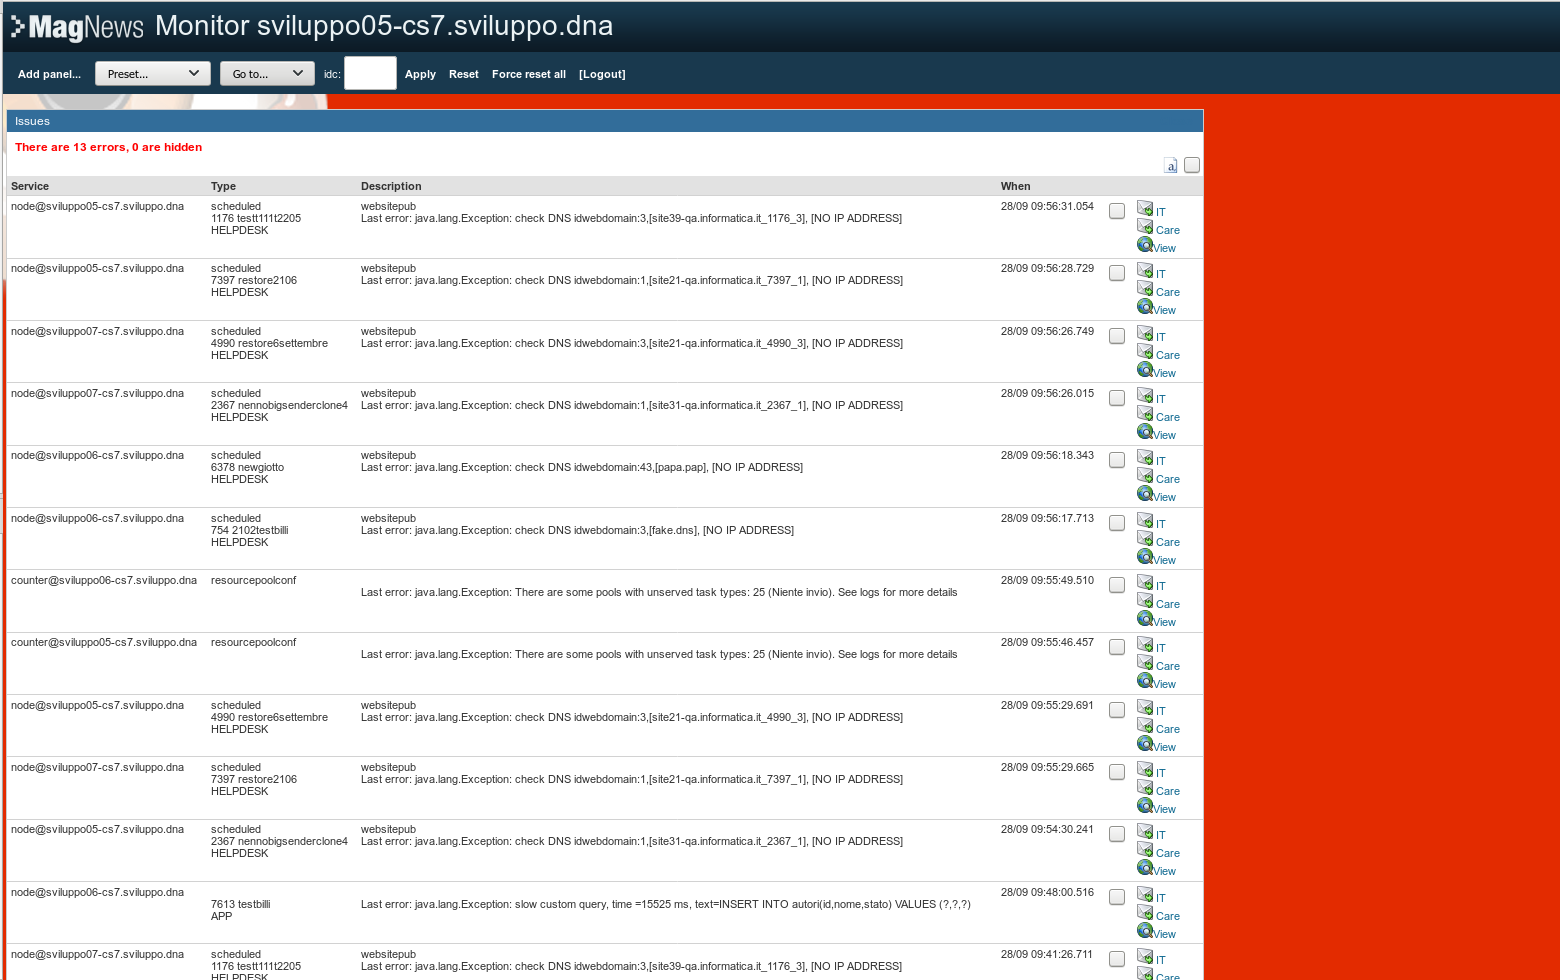
\includegraphics[width=\textwidth]{dashboard_old.png}
	\centering
\end{figure}
In questa figura si può notare che la dasboard è ricca di informazioni, molteplici segnalazioni
ma il contenuto è gestito male, organizzato in modo poco intuitivo e poco gradevole all'utilizzo.
Ogni tabella contiene migliaia di voci disordinate, e ogni pagina può contenere più tabelle
il che rende ancora più confusionario il tutto. Per migliorare tutto questo è stato inserimento
un framework grafico (\emph{Bootstrap}) e una libreria Javascript (\emph{DataTables}) che consentono
di maneggiare al meglio e in modo efficiente i componenti obsoleti utilizzati in precedenza.
Il risultato finale della home è questo:
\begin{figure}[H]
	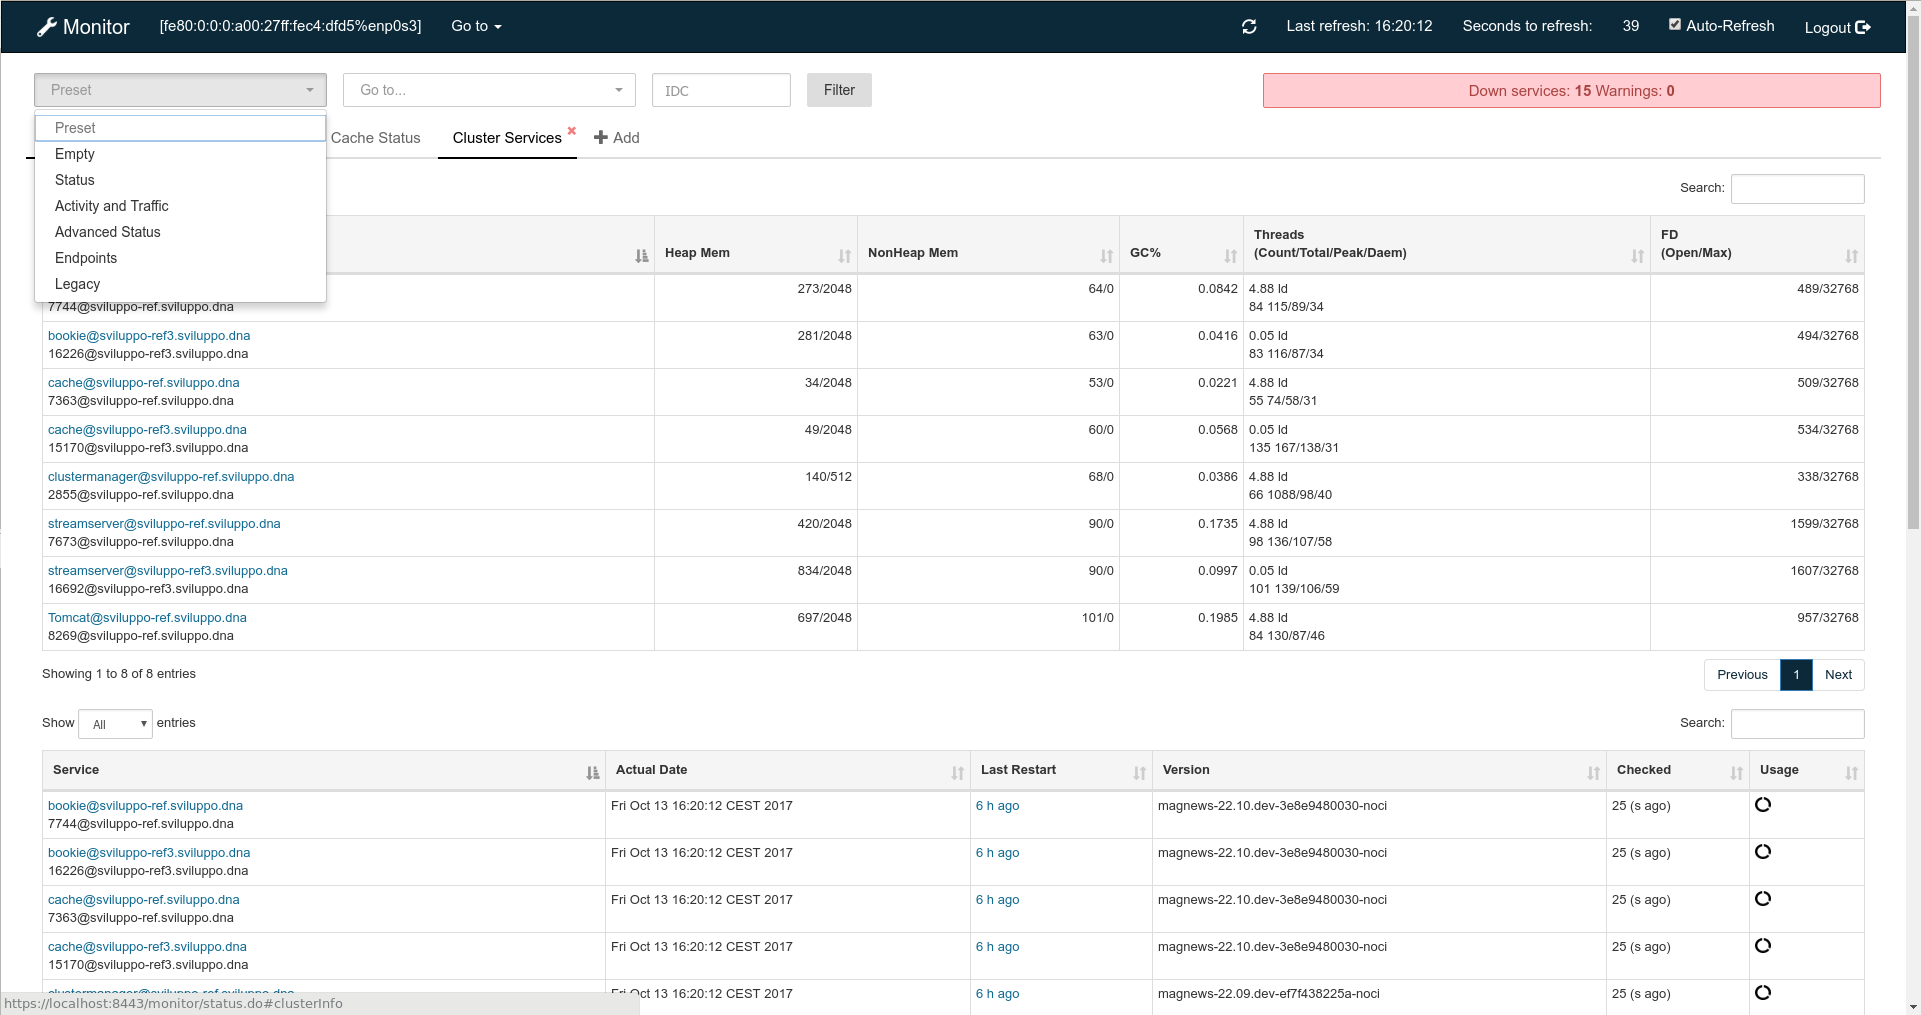
\includegraphics[width=\textwidth]{dashboard_new.png}
	\centering
\end{figure}
La navigazione ad altre pagine è più semplice, l'accesso ai warning e ai downservices
è più agevole e le tabelle sono completamente rinnovate vista l'introduzione della possibilità di
visualizzazione paginata e ordinamento.
\par Oltre ad aver cambiato la dashboard principale ho provveduto a far corrispondere schermate secondarie
che si rifanno allo stesso stile coerente con i colori del brand e l'immagine artistica del prodotto.\\
Per il login:
\begin{figure}[H]
	\centering
	\begin{subfigure}
	  \centering
	  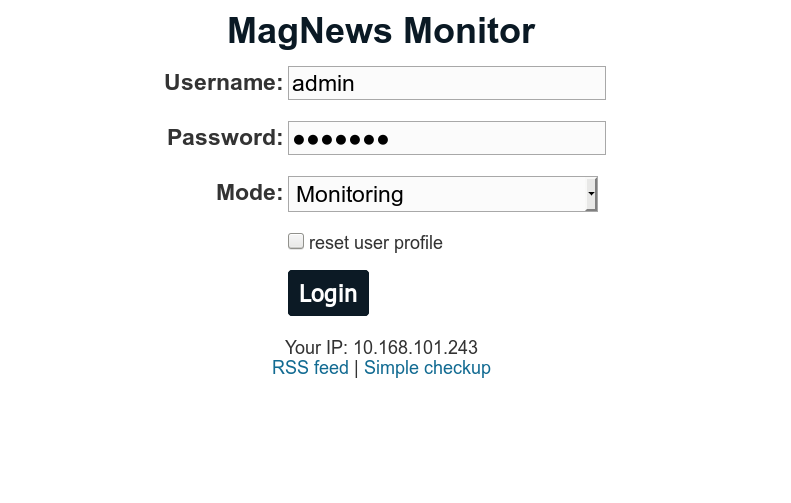
\includegraphics[width=0.45\linewidth]{login_old.png}
	\end{subfigure}%
	\begin{subfigure}
	  \centering
	  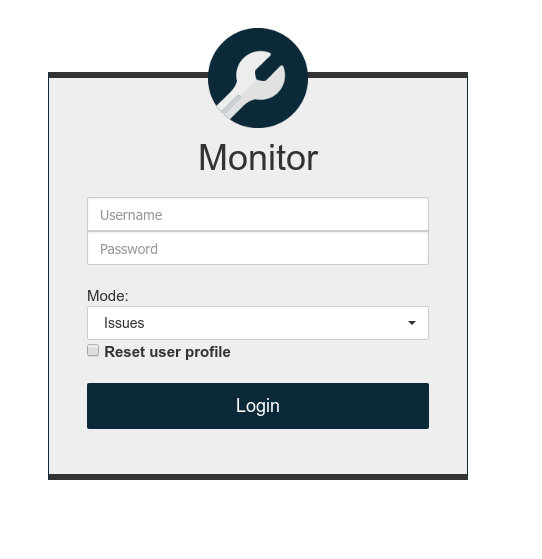
\includegraphics[width=0.45\linewidth]{login_new.png}
	\end{subfigure}
\end{figure}
Per una schermata secondaria fatta in Angular:
\begin{figure}[H]
	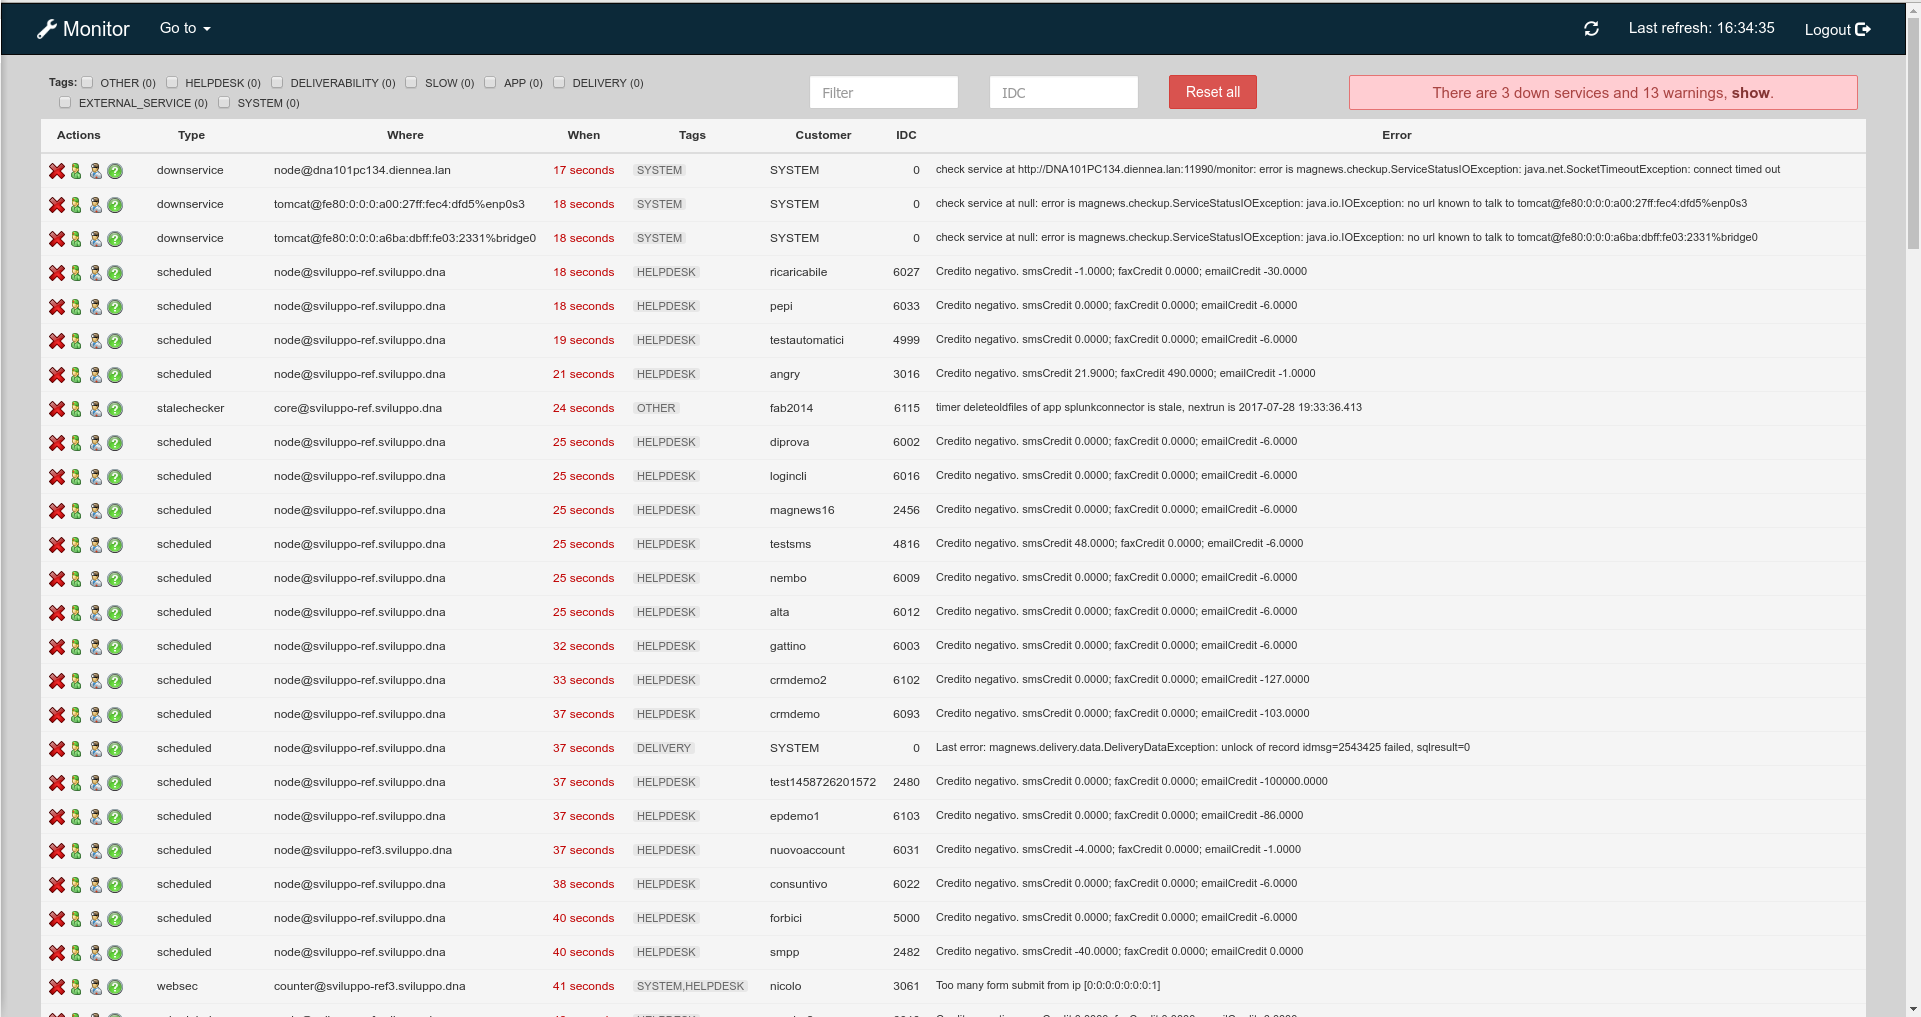
\includegraphics[width=\textwidth]{issue_new.png}
	\centering
\end{figure}

\par In questo modo si può filtrare, con query di ricerca, tutto quello che riguarda le colonne
e si possono visualizzare, anche in questa pagina, l'elenco dei servizi down con il 
riferimento a quanto tempo è che lo sono. 

\subsection{Risoluzione issues aziendali}
\par Durante lo sviluppo del prodotto, per mantenere il ritmo di rilascio mensile è 
ovviamente necessario che le persone che si occupano di quality assurance si occupino 
di mettere alla prova il programma in modo da averne un riscontro umano che va oltre
alle capacita dello Unit testing. Una parte molto importante, che fornisce input
ai developer sono gli \emph{issue}. Ovviamente questi input arrivano anche da segnalazioni
dei clienti oppure addirittura dai dev stessi che possono, allo stesso modo, fare richiesta
di segnalazione bug.\\
\par Inserirsi in un prodotto così ampio non è immediato, richiede tempo e studio.
Una comprensione completa non è possibile all'interno di un tirocinio curricolare, per
questi motivi mi sono stati assegnati principalmente tre issue prettamente formativi 
e mirati a farmi prendere dimestichezza con il progetto.
\par \textbf{Issue Aviary}: questo è un issue diviso in due parti: la parte di ricerca 
e analisi e la parte di aggiornamento. In breve Aviary è un \emph{SaaS} della famiglia
Adobe che fornisce gli strumenti necessari per la manipolazione di immagini attraverso
un editor posizionabile nel browser. Questo strumento verrà dismesso e non viene più
supportato dall'azienda. Questo implicava la ricerca di un sostituto e l'aggiornamento all'ultima versione.
Durante il progetto è stato sviluppato un piccolo prototipo di quello che sarà il successore.
Non sarà più un unico software ma l'unione di più librerie modulari che consentono di
ottenere un risultato più contenuto, intuitivo e mirato togliendo funzioni statisticamente
meno usate.\\
\par \textbf{Issue jQuery}: Buona parte delle animazioni è gestito da eventi jQuery 
dinamici che, alle volte, portano a bug di visualizzazione. Essendo numerosissime
le casistiche all'interno del codice, ho dedicato parecchie ore al fix di malfunzionamenti
logici, alla gestione di servizi di store di dati nella sessione e nel salvataggio di cookie.
Questo task, comprendeva anche los sviluppo di alcuni moduli \emph{Angular} e query live
che comunicavano con API Rest che prendevano i dati a loro volta dal backend Java.\\
\par \textbf{Issue Findbugs}: findbugs è uno dei plugin più utilizzati a build time 
per l'intercettazione e la correzione di possibili errori logici all'interno del codice.
Questo programma, come Aviary, non è più aggiornato ed ormai è obsoleto per le nuove
versioni di Java. Fortunatamente è stato fatto un fork chiamato \emph{SpotBugs}.
Questo fork essenzialmente si pone il goal di offrire le stesse funzionalità, nella
maniera più legacy possibile e portando avanti nuove feature.\\
Tutto questo, da parte mia è stato integrato alle \emph{dependency} e ai \emph{plugin}
Maven, e quindi è stato inserito nei file \emph{pom.xml}. In questo modo la build viene
eseguita con SpotBugs al posto di Findbugs. Questo task è stato formativo nei confronti
del build system Maven che è diverso da quello base Eclipse. Mette in gioco moltissime
funzionalità dinamiche di building del progetto e consente al programmatore di gestire
moduli, plugin, generazione di documentazione, unit testing e molto altro.
\\
\subsection{Rappresentazione grafica delivery}
\par Lo scopo principale di questo task era quello di creare una rappresentazione visuale
di quella che è la situazione della delivery aziendale delle mail. L'azienda spedisce
milioni di mail al giorno, molte delle quali fanno una coda di invio visti i costi 
computazionali dell'invio di così tanti dati. Molte mail vengono perse e quindi re-inviate.
Tutto questo processo è stato richiesto in una rappresentazione grafica su browser web.
I concetti chiave sono sicuramente le mail, la loro quantità, quando vengono richieste, quando
vengono effettivamente inviate e la quantità totale delle mail giornaliere.
\par Tutti questi dati sono stati immaginati graficamente come una pioggia di sfere (piene o vuote
in base a se si tratta di un invio di e-mail o SMS) che cadono durante il loro invio in un mare il cui
livello rappresenta il monte mail raggiunto nel giorno corrente. Il concept grafico è stato sviluppato
dall'UX designer in questo modo:
\begin{figure}[H]
	
\includegraphics[width=\textwidth]{Monitor.jpg}
	\centering
\end{figure}
\par Per fare in modo che il tutto prendesse forma ho sviluppato 2 parti diverse: la logica di modello,
la grafica in Javascript. Le classi di modello Javascript contengono un metodo che fa l'\emph{update}
e un metodo che fa il \emph{draw} della forma che rappresenta. Le palline sono sfere che possono 
collidere con il terreno che è formato da tasselli che aumentano l'altezza in base al 
valore di mail inviate. Le palline possono ``spawnare'' orizzontalmente come pioggia dal
cielo. La scritta incrementa il valore continuamente in base al valore che allo stesso tempo
indica il livello al terreno.
\par Per realizzare la parte grafica ho utilizzato la libreria Javascript \textbf{p5.js}.
Questa libreria mette a disposizione un controller con metodi di inizializzazione e game loop
per il disegno grafico. Mette a disposizione una libreria per le collisioni tra figure e la creazione
di figure castom attraverso curve di bezier e vertici.
\par Un'altra parte importante è l'ottenimento dei dati dal server. Per fare in modo che i dati
siano aggiornati si utilizza una logica polling temporizzata che chiede al server la situazione
ogni minuto partendo un minuto in ritardo. Con questo stratagemma si è a conoscenza della situazione della Mail
nel momento attuale e quello del minuto precedente. Fatto ciò si possono ottenere le informazioni
in modo leggere con un file JSON opportunamente creato e letto in modo nativo da Javascript.
Il risultato finale è molto simile a quello posto in partenza e tutt'ora è in via di sviluppo per 
quanto riguarda le animazioni e le migliorie grafiche.
\begin{figure}[H]
	
\includegraphics[width=\textwidth]{delivery-final.png}
	\centering
\end{figure}
\subsection{Workflow Git}
\par Una tra le cose più interessanti dell'andare in azienda è stato quello dell'inserirsi
nel workflow di un'azienda affermata che quotidianamente si trova di fronte a problemi,
task, feature e improvements da sviluppare. Tutto questo è scandito dal fatto che lo sviluppo
ha una tabella di marcia con date di release mensili ben definite.\\
Per questi motivi è necessario mantenere un ecosistema collaborativo, organizzato
al quale poter far riferimento durante la propria routine lavorativa.
Innanzitutto tutto il team fa utilizzo dell'ecosistema \emph{Atalassian Bitbucket}
on premise per mantenere il repository su un server locale sicuro ed affidabile.
Atalassian offre inoltre una priattaforma chiamata \emph{Jira} per pianificare, monitorare ed assegnare
ai dev compiti da svolgere e attività. \emph{Jira} è completamente in sinergia con
Bitbucket per quanto riguarda i commit riguardo quel branch di lavoro e per le code review 
del lavoro.
In azienda viene utilizzato \emph{Git} con un \emph{Feature Branch Workflow}.
Questo workflow è tipico dello sviluppo agile e ha la peculiarità di far lavorare
le persone su un branch dedicato alla feature e lasciare il master in uno stato funzionante
in modo da permettere di avere il programma intatto e le feature che lavorano in parallelo 
su branch che toccano parti di programma diverse.
\begin{figure}[H]
	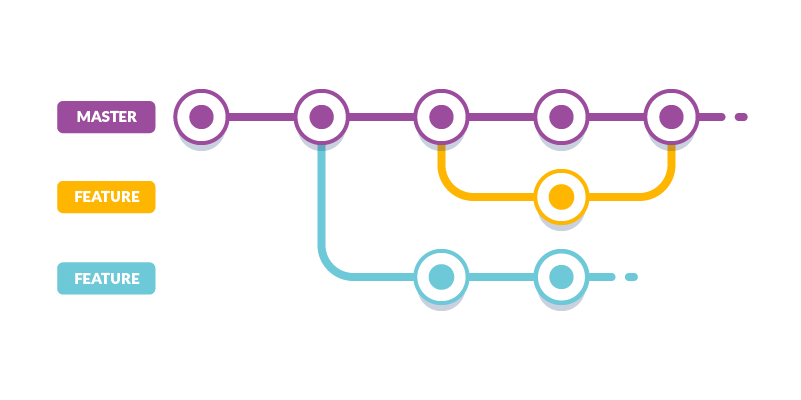
\includegraphics[width=0.8\textwidth]{feature-branch.png}
	\centering
\end{figure}
Solitamente ogni branch feature ha nome uguale (o che contiene il codice) dell'issue
a cui fa riferimento e ogni commit, allo stesso modo, contiene un codice univoco.
In questo modo la sincronizzazione è completa tra \emph{Jira} e \emph{Bitbucket} e quindi
di conseguenza tra organizzazione e sviluppo del codice.
Il solito iter di sviluppo è il seguente:
\begin{enumerate}
	\item Prendere in carico un issue segnalato.
	\item Creare un branch con il codice dell'issue.
	\item Fare i vari commit di sviluppo del branch.
	\item Fare un rebase del master e squash dei commit superflui.
	\item Attendere la code review del codice aggiunto.
	\item Integrare al master la feature terminata.
\end{enumerate}
\par In questa maniera e con queste particolari tecnologie lavorare in collaborazione
è più comodo, efficace e organizzato. Può causare eccessivi passaggi durante lo sviluppo
ma mantiene il tutto ``pulito'' e tracciato in modo da poter tornare indietro ad una
versione funzionante in ogni momento. 

\section{Conclusioni}
\par Alla fine delle 150 ore è stato prodotto il frontend di un monitor, sono stati
sistemati bug del prodotto e analizzati diversi framework al fine di avviare un
processo di rework completo che potrebbe durare anche parecchi mesi. Reputo positivo il risultato
visto che si tratta di un progetto molto vasto e complesso.
\par In conclusione è stata una esperienza nel complesso positiva. Ha avuto alti e bassi in quanto 
a mole di lavoro e produttività. Nei momenti lati includerei la grande quantità
di esperienza acquisita a contatto con senior developers, esperienza di quella che è
la modalità di lavoro in collaborazione e la vasta copertura tecnologica all'interno
dell'azienda. Nei lati negativi inserirei assolutamente la difficoltà in un tirocinio
di 150 ore ad inserirsi in un progetto di quella complessità riuscendo ad avere un 
impatto vero e proprio. \\
Questo tipo di esperienza ti apre gli occhi sul mondo del lavoro ma allo stesso tempo
ti fa realizzare che in ambito informatico l'orizzonte è ampio e c'è una vasta disomogeneità
su quella che è la conoscenza richiesta.

\renewcommand{\refname}{Bibliografia}
\begin{thebibliography}{9}
  \bibitem{latexcompanion} 
  Michel Goossens, Frank Mittelbach, and Alexander Samarin. 
  \textit{The \LaTeX\ Companion}. 
  Addison-Wesley, Reading, Massachusetts, 1993.
   
  \bibitem{einstein} 
  Albert Einstein. 
  \textit{Zur Elektrodynamik bewegter K{\"o}rper}. (German) 
  [\textit{On the electrodynamics of moving bodies}]. 
  Annalen der Physik, 322(10):891–921, 1905.
   
  \bibitem{knuthwebsite} 
  Knuth: Computers and Typesetting,
  \\\texttt{http://www-cs-faculty.stanford.edu/\~{}uno/abcde.html}
  \end{thebibliography}

\end{document}